\section{A new upper bound for the de Bruijn-Newman constant}\label{newup-sec}

In this section we prove Theorem \ref{new-upper}. 

\subsection{Selection of parameters}\label{select}

As stated in the introduction, it suffices to verify the conditions (i), (ii), (iii) of Theorem \ref{ubc-0} $t_0 \coloneqq 0.2$, $X \coloneqq X_0-0.5$, and $y_0 \coloneqq 0.2$, where $X_0 \coloneqq 6 \times 10^{10} + 83952$.  

The choice $t_0=y_0=0.2$ is due to the limitations of our numerical verifications, particularly the known numerical verification of RH.  We now explain the choice of $X_0$.  Recall the familiar Euler product factorization
$$ \zeta(s) = \prod_p \left(1 - \frac{1}{p^s}\right)^{-1}$$
for the Riemann zeta function.  This leads to the heuristic
$$ H_0(x+iy) \propto \prod_{p \leq P} \left(1 - \frac{1}{p^s}\right)^{-1}$$
for some small prime cutoff $P$, where $s = \frac{1+y+ix}{2}$ and we are extremely vague as to what the proportionality symbol $\propto$ means.  This heuristic extends to non-zero times $t$ as
$$ H_t(x+iy) \propto \prod_{p \leq P} \left(1 - \frac{b_n^t}{p^s}\right)^{-1}$$
and we also have
\begin{equation}\label{oscil}
 f_t(x+iy) \propto \prod_{p \leq P} \left(1 - \frac{b_n^t}{p^s}\right)^{-1}.
\end{equation}
One can non-rigorously justify the latter assertion by by inspecting the first series of $f_t(x+iy)$ in \eqref{ft-def} and ignoring the fact that the sequence $n \mapsto b_n^t$ is not multiplicative when $t \neq 0$.  

We will be relying heavily on Corollary \ref{zero-test}, and therefore seek to ensure that $|f_t(x+iy)|$ is as large as possible.
It would therefore seem to be advantageous to try to work as much as possible in regions where Euler product
$$ \prod_{p \leq P} \left(1 - \frac{b_n^t}{p^s}\right),$$
is small, which heuristically corresponds to $\frac{x}{4\pi} \log p$ being close to an integer for $p \leq P$ (so that $p^s$ has argument close to zero).  If one chooses $x$ to lie in the vicinity of
$$ X \coloneqq 6 \times 10^{10} + 83952 - 0.5$$
then indeed the fractional parts $\{ \frac{X}{4\pi} \log p\}$ for $p \leq 11$ are somewhat close to zero:
\begin{align*}
\{ \frac{X}{4\pi} \log 2 \} &= 0.0275\dots \\
\{ \frac{X}{4\pi} \log 3 \} &= 0.0437\dots \\
\{ \frac{X}{4\pi} \log 5 \} &= 0.0640\dots \\
\{ \frac{X}{4\pi} \log 7 \} &= 0.0774\dots\\
\{ \frac{X}{4\pi} \log 11 \} &= 0.0954\dots
\end{align*}
We found this shift by the following somewhat \emph{ad hoc} procedure.  We first introduced the quantity
$$ \mathrm{eulerprod}(x,p_n) \coloneqq \left|\prod\limits_{p \leq p_n}\frac{1}{1-\frac{1}{p^{1-ix/2}}}\right|,$$
which is the  exponent corresponding to $y=1$ (where the minimum value of $|f_t(x+iy)|$ in the barrier region is expected to occur).  We numerically located candidate integers $1 \leq q \leq 10^5$ for which the quantity
$$ \min_{x - 6 \times 10^{10} - q \in \{-0.5,0,0.5\}} |\mathrm{eulerprod}(x,29)|$$
exceeded a threshold (we chose $4$), to obtain seven candidates for $q$: $1046$, $22402$, $24198$, $52806$, $77752$, $83952$, and $99108$.  Among these candidates, we selected the value of $q$ which maximised the quantity
$$ \min_{x - 6 \times 10^{10} - q \in \{-0.5,0,0.5\}} |f_0(x+i)|,$$
namely $q = 83952$ (this quantity being $\approx 4.32$ for this value of $q$).
\begin{figure}[h!]
  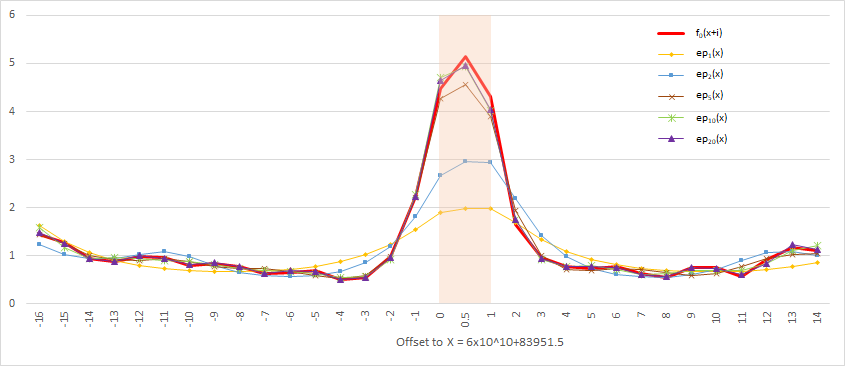
\includegraphics[width=\linewidth]{euler_product_approximation.png}
  \caption{Improving approximation of $\mathrm{ep}_n(x)$ w.r.t. $|f_0(x+iy)|$ as $n$ is increased, where $\mathrm{ep}_n(x)=\mathrm{eulerprod}(x,p_n)$, shown near $X=6 \times 10^{10} + 83951.5$, which was chosen as a barrier location.}
	\label{euler}
\end{figure}




\subsection{Verifications of claims}

Claim (i) of Theorem \ref{ubc-0} is immediate from the result of Platt \cite{platt} that all the non-trivial zeroes of $\zeta$ with imaginary part between $0$ and $3.06 \times 10^{10}$ lie on the critical line $\{ \mathrm{Re}(s) = 1/2\}$.  For the remaining claims (ii), (iii) of Theorem \ref{ubc-0}, it will suffice to verify that $H_t(x+iy) \neq 0$ for the following three regions of $(x,y,t)$:
\begin{itemize}
\item[(ii)]  $x \geq X_0 - 0.5 + \sqrt{0.96}$, $0.2 \leq y \leq \sqrt{0.6}$, and $t = 0.2$. 
\item[(iii)]  $X_0 - 0.5 \leq x \leq X_0 + 0.5$, $0.2 \leq y \leq \sqrt{0.6}$, and $0 \leq t \leq 0.2$.
\end{itemize}
Here we have enlarged the region (iii) for simplicity.  Both of these regions lie in \eqref{region}.  We can of course replace $H_t(x+iy)$ by $H_t(x+iy)/B_t(x+iy)$.  

Set
$$ N \coloneqq \left\lfloor \sqrt{\frac{x}{4\pi} + \frac{t}{16}} \right\rfloor $$ % \leq \left(\frac{x}{4\pi} (1 + \frac{\pi t}{4x})\right)^{1/2},$$
so in particular
%\begin{equation}\label{logx}
 %\log \frac{x}{4\pi} \geq 2 \log N - \log(1 + \frac{\pi t}{4x}).
%\end{equation}
%Also we have
\begin{equation}\label{xnn}
 x_N \leq x < x_{N+1}
\end{equation}
where
$$ x_N \coloneqq 4 \pi N^2 - \frac{\pi t}{4}.$$
Write $N_0 \coloneqq 69098$ and $N_1 \coloneqq 1.5 \times 10^6$.
In region (ii) we then have $N = N_0$, while in region (iii) we have $N \geq N_0$.  It will now suffice to verify $\frac{H_t(x+iy)}{B_t(x+iy)} \neq 0$ in the following three regions:
\begin{itemize}
\item[(a)]  When $X_0 - 0.5 \leq x \leq X_0 + 0.5$, $N = N_0$, $0 \leq t \leq 0.2$, and $0.2 \leq y \leq 1$.
\item[(b)]  When $x \geq X_0 - 0.5$, $N_0 \leq N \leq N_1$, $t = 0.2$, and $0.2 \leq y \leq 1$.
\item[(c)]  When $N \geq N_1$, $t = 0.2$, and $0.2 \leq y \leq 1$.
\end{itemize}

In all three regions we use the following approximation:

\begin{proposition}\label{sweep}  Let $(x,y,t)$ lie in one of the regions (a), (b), (c).
Define
\begin{align*}
f_t(x+iy) &\coloneqq \sum_{n=1}^N \frac{b_n^t}{n^{s_*}} + \gamma \sum_{n=1}^N n^y \frac{b_n^t}{n^{\overline{s_*} + \kappa}}\\
b_n^t &\coloneqq \exp( \frac{t}{4} \log^2 n),\\
\end{align*}
where $\kappa, s_*, \gamma$ are as in Theorem \ref{eff}.  Then
\begin{equation}\label{bbb}
\frac{H_t(x+iy)}{B_t(x+iy)} = f_t(x+iy) + O_{\leq}( 1.25 \times 10^{-3} ).
\end{equation}
\end{proposition}

\begin{proof} 
By Theorem \ref{eff} it suffices to show that
$$ e_A + e_B + e_{C,0} \leq 1.25 \times 10^{-3}.$$
From Theorem \ref{eff} again, we have
\begin{equation}\label{eaeb-bound}
 e_A + e_B \leq (e^{\delta_1}-1) (F_{N,t}(\mathrm{Re}(s_*)) + |\gamma| F_{N,t}( \mathrm{Re}(s_*) - y - |\kappa| ) )
\end{equation}
where
\begin{equation}\label{fnt-def}
 F_{N,t}( \sigma ) := \sum_{n=1}^N \frac{b_n^t}{n^\sigma}.
\end{equation}
and
\begin{equation}\label{dela}
 \delta_1 \coloneqq \frac{\frac{t^2}{16} \log^2 \frac{x}{4\pi} + 0.626}{x-6.66}.
\end{equation}
From Lemma \ref{elem-lem}(vi), the quantity $\delta_1$ is monotone decreasing in $x$ in the region \eqref{region}.  Thus we have
\begin{equation}\label{delta1-bound}
 \delta_1 \leq \frac{\frac{(0.2)^2}{16} \log^2 \frac{X_0-0.5}{4\pi} + 0.626}{X_0-0.5-6.66}
\end{equation}
whenever $x \geq X_0-0.5 \geq 200$ and $0 \leq t \leq 0.2$.  Computing the right-hand side, we conclude that
$$  \delta_1 \leq 3.12 \times 10^{-11}$$
and hence by Taylor expansion
$$ e^{\delta_1} - 1 \leq 1.001 \delta_1$$
(say).
Also, from Theorem \ref{eff} and \eqref{fnt-def} we can bound
\begin{align*}
|\gamma| F_{N,t}( \mathrm{Re}(s_*) - y - |\kappa| ) &\leq |\gamma| N^y N^{|\kappa|} F_{N,t}( \mathrm{Re}(s_*) ) \\
&\leq \exp\left( 0.02 y + y \left(\log N - \frac{1}{2} \log \frac{x}{4\pi}\right) + \frac{ty}{2(x-6)} \log N \right) F_{N,t}( \mathrm{Re}(s_*) )  \\
&\leq \exp\left( 0.02 y + \left(y + \frac{ty}{2(x-6)}\right) \frac{1}{2} \log(1 + \frac{\pi t}{4x}) + \frac{ty}{4(x-6)} \log \frac{x}{4\pi} \right) F_{N,t}( \mathrm{Re}(s_*) ).
\end{align*}
For $0.2 \leq y \leq 1$, $0 \leq t \leq 0.2$, and $x \geq X_0 - 0.5$ we see from Lemma \ref{elem-lem}(vi) that
$$ \frac{ty}{4(x-6)} \log \frac{x}{4\pi} \leq \frac{0.2}{4(X_0 - 0.5-6)}\log \frac{X_0 - 0.5}{4\pi} \leq 1.86 \times 10^{-11}$$
and
$$ \left(y + \frac{ty}{2(x-6)}\right) \frac{1}{2} \log(1 + \frac{\pi t}{4x}) \leq \left(1 + \frac{0.2}{2(X_0-0.5-6)}\right) \frac{1}{2} \log\left(1 + \frac{0.2 \pi}{4(X_0-0.5)}\right) \leq 1.31 \times 10^{-12}$$
and thus
\begin{equation}\label{gafn}
 |\gamma| F_{N,t}( \mathrm{Re}(s_*) - y - |\kappa| ) \leq 1.021  F_{N,t}( \mathrm{Re}(s_*) ).
\end{equation}
Thus
$$  e_A + e_B \leq 1.023 \delta_1 F_{N,t}( \mathrm{Re}(s_*) ).$$
To estimate $\mathrm{Re}(s_*)$, we use Proposition \ref{estimates}(ii) or \eqref{kappa-bound}, together with the inequality
$$ \frac{t}{2x^2} \left(1-3y+\frac{4y(1+y)}{x^2}\right)_+ \leq \frac{0.2}{2 (X_0-0.5)^2} \left(1 - 3 \times 0.2 + \frac{8}{(X_0-0.5)^2}\right)_+
\leq 1.2 \times 10^{-23}$$
to obtain 
$$ \mathrm{Re}(s_*) \geq 0.6001 + \frac{t}{4} \log \frac{x}{4\pi}$$
(say).  Since $F_{N,t}(\sigma)$ is non-increasing in $\sigma$, we conclude
$$  e_A + e_B \leq 1.023 \delta_1 F_{N,t}\left( 0.6001 + \frac{t}{4} \log \frac{x}{4\pi} \right).$$
Since
$$ N = \left\lfloor \sqrt{\frac{x}{4\pi} + \frac{t}{16}} \right\rfloor,$$
$0 \leq t \leq 0.2$, and $x \geq X_0-0.5$, it is easy to see that
$$ N \leq \frac{x}{4\pi}$$
and hence by \eqref{bn-def}
$$ \frac{b_n^t}{n^{\frac{t}{4} \log \frac{x}{\pi}}} \leq 1$$
for all $1 \leq n \leq N$.  Therefore
$$ F_{N,t}\left( 0.6001 + \frac{t}{4} \log \frac{x}{4\pi} \right) \leq \sum_{n=1}^N \frac{1}{n^{0.6001}}$$
and hence by the integral test
$$ F_{N,t}\left( 0.6001 + \frac{t}{4} \log \frac{x}{4\pi} \right) \leq \int_1^{N+1} \frac{ds}{s^{0.6001}} = \frac{1}{0.3999} (N+1)^{0.3999} $$
so that (by \eqref{dela})
$$ e_A + e_B \leq 1.023 \frac{\frac{(0.2)^2}{16} \log^2 \frac{x}{4\pi} + 0.626}{x-6.66} \frac{1}{0.3999} (N+1)^{0.3999}.$$
We have
$$ N+1 \leq (1.001) \left(\frac{x-6.66}{4\pi}\right)^{1/2} $$
(say), and hence
$$ e_A + e_B \leq 0.7220 \frac{0.0025 \log^2 \frac{x}{4\pi} + 0.626}{(x-6.66)^{0.79995}}$$
From Lemma \ref{elem-lem}(vi), the right-hand side is monotone decreasing in the region $x \geq X_0-0.5$, thus
\begin{align*}
 e_A + e_B &\leq 0.7220 \frac{0.0025 \log^2 \frac{X_0-0.5}{4\pi} + 0.626}{(X_0-0.5-6.66)^{0.79995}} \\
&\leq 3.444 \times 10^{-9}.
\end{align*}

Meanwhile, from Proposition \ref{estimates}(vi) one has
$$ e_{C,0} \leq \left(\frac{x}{4\pi}\right)^{-\frac{1+y}{4}} \exp\left( - \frac{t}{16} \log^2 \frac{x}{4\pi} + \frac{3 |\log \frac{x}{4\pi} + i \frac{\pi}{2}|+3.58}{x-8.52} \right) \left(1 + \frac{1.24 \times (3^y+3^{-y})}{N-0.125} + \frac{6.92}{x-6.66}\right).$$
From Lemma \ref{elem-lem}(vi), the quantity $\frac{\log^2 \frac{x}{4\pi} + \frac{\pi^2}{4}}{(x-8.52)^2}$ is monotone decreasing in $x$ in \eqref{region}, hence $\frac{|\log \frac{x}{4\pi} + i \frac{\pi}{2}|}{x-8.52}$ is also monotone decreasing.  Also the expression is monotone decreasing in $y$. We conclude that
\begin{equation}\label{ec0-bound}
\begin{split}
 e_{C,0} &\leq \left(\frac{X_0-0.5}{4\pi}\right)^{-\frac{1+0.2}{4}} \exp\left( \frac{3 |\log \frac{X_0-0.5}{4\pi} + i \frac{\pi}{2}|+3.58}{X_0-0.5-8.52} \right) \left(1 + \frac{1.24 \times (3^{\sqrt{0.6}}+3^{-\sqrt{0.6}})}{N_0-0.125} + \frac{6.92}{X_0-0.5-6.66}\right) \\
&\leq 1.249 \times 10^{-3}
\end{split}
\end{equation}
where we have discarded the negative term $- \frac{t}{16} \log^2 \frac{X_0-0.5}{4\pi}$.  Combining the estimates, we obtain the claim.
\end{proof}

Now we attend to the three claims.


\subsection{Proof of claim (c)}\label{c-bound}  

We begin with claim (c), which is the easiest.  
By Proposition \ref{sweep}, it suffices to establish the bound
$$ |f_t(x+iy)| > 1.25 \times 10^{-3}.$$
In fact we will establish the stronger estimate
\begin{equation}\label{ft0}
f_t(x+iy) = 1 + O_{\leq}( 0.955 ).
\end{equation}

In the region (c) we have from \eqref{xnn} that
$$ x \geq x_{N_1} \geq  2.82 \times 10^{13}.$$

Our main tool here is the triangle inequality.  From \eqref{ft-def} one has
$$
f_t(x+iy) = 1 + \sum_{n=2}^N \frac{b_n^t}{n^{s_*}} + \gamma \sum_{n=1}^N n^y \frac{b_n^t}{n^{\overline{s_*} + \kappa}}$$
and hence
$$ f_t(x+y) = 1 + O_{\leq}\left( \sum_{n=2}^N \frac{b_n^t}{n^{\sigma}} + |\gamma| \sum_{n=1}^N n^y \frac{b_n^t}{n^{\sigma + |\kappa|}} \right)$$
where $\sigma \coloneqq \mathrm{Re} s_*$.  Restoring the $n=1$ term in the first sum and recalling that $t=0.2$, it thus suffices to show that
\begin{equation}\label{nan}
 \sum_{n=1}^N \frac{b_n^{0.2}}{n^\sigma} + |\gamma| \sum_{n=1}^N n^y \frac{b_n^{0.2}}{n^{\sigma-|\kappa|}}
< 1.955.
\end{equation}
Our main tool here will be 

\begin{lemma}\label{largen}
Let $N \geq N_0 \geq 1$ be natural numbers, and let $\sigma,t > 0$ be such that
$$ \sigma > \frac{t}{2} \log N.$$
Then
$$ \sum_{n=1}^N \frac{b_n^t}{n^\sigma} \leq \sum_{n=1}^{N_0}
\frac{b_n^t}{n^\sigma}  + 
\max( N_0^{1-\sigma} b_{N_0}^t, N^{1-\sigma} b_N^t ) \log \frac{N}{N_0}.$$
\end{lemma}

\begin{proof}  From the identity
$$ \frac{b_n^t}{n^\sigma} = \frac{\exp\left( \frac{t}{4} (\log N - \log n)^2 - \frac{t}{4} (\log N)^2\right) }{n^{\sigma - \frac{t}{2} \log N}}$$
we see that the summands $\frac{b_n^t}{n^\sigma}$ are decreasing for $1 \leq n \leq N$, hence by the integral test one has
\begin{equation}\label{rado}
 \sum_{n=1}^N \frac{b_n^t}{n^\sigma} \leq \sum_{n=1}^{N_0}
\frac{b_n^t}{n^\sigma}  + \int_{N_0}^N \frac{b_a^t}{a^\sigma}\ da.
\end{equation}
Making the change of variables $a = e^u$, the right-hand side becomes
$$\sum_{n=1}^{N_0} \frac{b_n^t}{n^\sigma} \exp( (1-\sigma) u + \frac{t}{4} u^2 )\ du.$$
The expression $(1-\sigma) u + \frac{t}{4} u^2$ is convex in $u$, and is thus bounded by the maximum of its values at the endpoints $u = \log N_0, \log N$; thus
$$\exp( (1-\sigma) u + \frac{t}{4} u^2) \leq N_0^{1-\sigma} b_{N_0}^t, N^{1-\sigma} b_N^t.$$
The claim follows. 
\end{proof}

\begin{remark}  The right-hand side of \eqref{rado} can be evaluated exactly as
$$
\sum_{n=1}^{N_0}
\frac{b_n^t}{n^\sigma}  + \frac{\sqrt \pi}{\sqrt t} \exp(\frac{-(\sigma - 1)^2}{t}) \left( \operatorname{erfi}\left(\frac{\frac{t}{2} \log N  - \sigma + 1}{\sqrt t} \right) - \operatorname{erfi}\left(\frac{\frac{t}{2} \log N_0  - \sigma + 1}{\sqrt t}\right) \right).$$

In practice, this upper bound for $\sum_{n=1}^N \frac{b_n^t}{n^\sigma}$ is slightly more accurate than the one in Lemma \ref{largen}, and is a good approximation even for relatively small values of $N_0$ (e.g., $N_0=100$).  However, the cruder bound above suffices for the numerical values of parameters needed to establish the bound $\Lambda \leq 0.22$.
\end{remark}

Observe from \eqref{kappa-bound} that
$$ |\kappa| \leq \frac{0.2 \times 0.2}{2(2.82 \times 10^{13}-6)} \leq 7.08 \times 10^{-16}$$
while from \eqref{gamma-bound} one has
$$
|\gamma| \leq 1.005 \left( \frac{x_N}{4\pi} \right)^{-y/2}$$
so in particular since $0.2 \leq y \leq 1$ and $n \leq 1.0001 (\frac{x_N}{4\pi})^{1/2}$
$$
|\gamma| n^y \leq 1.006 \left( \frac{x_N}{4\pi} \right)^{-0.1} n^{0.2}.$$
Also from \eqref{res-bound} one has
\begin{align*}
\sigma &\geq 0.6 + \frac{0.2}{4} \log \frac{x_N}{4\pi} - \frac{0.2}{2x_{N_1}^2} \left(0.4+\frac{0.96}{x_{N_1}^2}\right)_+ \\
&\geq 0.6 + 0.1 \log N + 0.05 \log \left(1 - \frac{t}{16 (N_1)^2}\right) - \frac{0.2}{2x_{N_1}^2} \left(0.4+\frac{0.96}{x_{1.5\times 10^6}^2}\right)_+ \\
&\geq 0.6 + 0.1 \log N - 5.1 \times 10^{-29}.
\end{align*}
We can then apply Lemma \ref{largen} twice to bound the left-hand side of \eqref{nan} by $A+B$, where
\begin{align*}
A &\coloneqq \sum_{n=1}^{N_0} \frac{b_n^{0.2}}{n^{\sigma'}} + 1.006 \left( \frac{x_N}{4\pi} \right)^{-0.1} \sum_{n=1}^{N_0} \frac{b_n^{0.2}}{n^{\sigma''}}, \\
B &\coloneqq (\max( N_0^{1-\sigma'} b_{N_0}^{0.2}, N^{1-\sigma'} b_N^{0.2} ) + 1.006 \left( \frac{x_N}{4\pi} \right)^{-0.1} 
\max( N_0^{1-\sigma''} b_{N_0}^{0.2}, N^{1-\sigma''} b_N^{0.2} ) )\log \frac{N}{N_0} \\
\sigma' &:= 0.6 + 0.1 \log N - 5.1 \times 10^{-29} \\
\sigma'' &:= 0.4 + 0.1 \log N - 7.09 \times 10^{-16}.
\end{align*}
The quantity $A$ is decreasing in $N$, so we may bound it by its value at $N = N_1$.  Performing the sum numerically, we obtain
$$ A \leq 1.88.$$
Finally, the quantity $B$ can also be seen to be decreasing in $N$ in the range $N \geq N_1$, and obeys the bound
$$ B \leq 0.075.$$
The claim follows.

\begin{figure}[h!]
  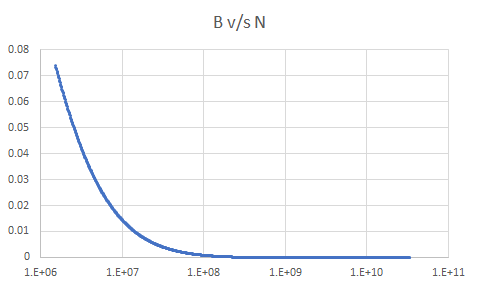
\includegraphics[width=0.7\linewidth]{B_vs_N.png}
  \caption{Plot of $B$ vs $N$}
\end{figure}


\subsection{Proof of claim (a)}\label{barrier-sec}

For region (a) we again verify \eqref{ft0}.
As $N = N_0$ is constant in this region, the function $f_t(x+iy)$ is holomorphic, so by Rouche's theorem, it suffices to show that for each time $0 \leq t \leq 0.2$, as $x+iy$ traverses the boundary $\partial R$ of the rectangle 
$$ R \coloneqq \{ x+iy: X_0 - 0.5 \leq x \leq X_0 + 0.5; 0.2 \leq y \leq 1 \},$$
the function $f_t(x+iy)$ stays outside of the ball $B \coloneqq \{ z: |z| \leq 1.25 \times 10^{-3} \}$, and furthermore has a winding number of zero around the origin.

To verify this claim numerically for a given value of $t$, we subdivide each edge of $\partial R$ into some number $n$ of equally spaced mesh points, thus approximating $\partial R$ by a discrete mesh $x_j+iy_j$, $j=1,\dots,4n$, with any two adjacent points on this mesh separated by a distance at most $1/n$.  Using the techniques in Section \ref{multiple-sec}, we evaluate $f_t(x_j+iy_j)$ numerically for each such value of $j$.  The polygonal path connecting these points then winds around the origin with winding number
$$ \frac{1}{2\pi} \sum_{j=1}^{4n} \mathrm{arg}( f_t(x_{j+1}+iy_{j+1}) / f_t(x_j + i y_j) )$$
which can be easily computed (and verified to be zero).  To pass from this polygonal path to the true trajectory $f_t(\partial R)$ of $f_t(x+iy)$ on $\partial R$, we again use Rouche's theorem.  If one has a derivative bound $|\frac{\partial}{\partial z} f_t(z)| \leq D_z$ on the boundary of the rectangle, the polygonal path and the true trajectory $f_t(\partial R)$ differ by a distance of at most $\frac{D_z}{2n}$, and the latter will have the same winding number around the origin (and stay outside of the ball $B$) as long as
$$ |f_t(x_j + iy_j)| > 1.25 \times 10^{-3} + \frac{D_z}{2n}.$$
Furthermore, the same is true for nearby times $t \leq t' \leq 0.2$ to $t$, as long as one has the stronger bound
\begin{equation}\label{cond}
 |f_t(x_j + iy_j)| > 1.25 \times 10^{-3} + \frac{D_z}{2n} + \frac{D_t |t'-t|}{2n}
\end{equation}
and a bound of the form $|\frac{\partial}{\partial t} f_{\tilde t}(z)| \leq D_t$
for $t \leq \tilde t \leq 0.2$ and $z \in \partial R$.

This gives the following algorithm to verify (i) for the entire range $0 \leq t \leq 0.2$.  We start with $t=0$ and obtain bounds $D_t, D_z$ for the derivatives of $f_{\tilde t}(z)$ in the indicated ranges.  Because of the way the barrier location $X$ was selected, we expect $|f_t(x+iy)|$ to stay well above $1$ in magnitude.  We thus choose $n$ so that $\frac{D_z}{2n} \leq 1$, and evaluate $f_t(x_j+iy_j)$ at all the mesh points (in particular confirming that $|f_t(x_j+iy_j)|$ does stay well above $1$).  Using the minimum value of $|f_t(x_j+iy_j)|$, we can then use the condition \eqref{cond} to establish the claim for times in the interval $[t,t')$ where $t'>t$ is chosen so that \eqref{cond} holds (or $t'=0.2$, if that is also possible); the most aggressive choice of $t'$ would be one in which \eqref{cond} held with equality, but in practice we can afford to take more conservative values of $t'$ and still obtain good runtime performance.  If $t' < 0.2$, we then repeat the process, replacing $t$ by $t'$, until the entire range $0 \leq t \leq 0.2$ is verified.

To run this algorithm, we need bounds on $D_t$ and $D_z$.  This is achieved by the following lemma, which gives bounds which are somewhat complicated but which can be easily upper bounded numerically on $\partial R$:

\begin{lemma} In the region \eqref{region}, and away from the jump discontinuities of $N$, we have
\begin{align*}
 \left|\frac{\partial f_t}{\partial z}\right| &\leq  \sum_{n=1}^N \frac{b_n^t}{n^{\mathrm{Re}(s_*)}} \left(\frac{\log n}{2} + \frac{t \log n}{4(x-6)}\right) \\
&\quad + |\gamma| N^{|\kappa|} \sum_{n=1}^N \frac{b_n^t n^{y} }{n^{\mathrm{Re}(s_{*})}}
\left( \frac{t \log n}{4(x-6)} + \left(\log \frac{|1+y+ix|}{4\pi} + \pi + \frac{3}{x}\right) \left(\frac{1}{2} + \frac{t}{4(x-6)}\right)\right)
\end{align*}
and
\begin{align*} \left|\frac{\partial f_t}{\partial t}\right| &\leq \sum_{n=1}^N \frac{b_n^t}{n^{\mathrm{Re} s_*}} \left(\frac{1}{4} \log n \log \frac{x}{4\pi n} + \frac{\pi}{8} \log n + \frac{2 \log n}{x-6}\right) \\
&\quad + |\gamma| N^{|\kappa|} \sum_{n=1}^N \frac{b_n^t n^y}{n^{\mathrm{Re}(s_{*})}}
\left(\frac{1}{4} \log n \log \frac{x}{4\pi n} + \frac{\pi}{8} \log n + \frac{2 \log n}{x-6} + \frac{1}{4} \left(\frac{\pi}{2} + \frac{8}{x-6}\right) \left(\log \frac{x}{4\pi} + \frac{8}{x-6}\right)\right).
\end{align*}
\end{lemma}

\begin{proof}
We begin with the first estimate.  Write 
$$ s_{**} \coloneqq \overline{s_*} - y + \kappa = \frac{1-y+ix}{2} + \frac{t}{2} \alpha\left(\frac{1-y+ix}{2}\right)$$
then
\begin{equation}\label{ftne}
f_t = \sum_{n=1}^N \frac{b_n^t}{n^{s_*}} + \gamma \sum_{n=1}^N \frac{b_n^t}{n^{s_{**}}}.
\end{equation}
One can check that $s_*, s_{**}, \gamma$ are holomorphic functions of $x+iy$, hence by the Cauchy-Riemann equations
$$ \left|\frac{\partial f_t}{\partial x}\right| = \left|\frac{\partial f_t}{\partial y}\right|.$$
By the product and chain rules, we may calculate
$$ 
\frac{\partial f_t}{\partial x} = - \sum_{n=1}^N \frac{b_n^t}{n^{s_*}} \frac{\partial s_*}{\partial x} \log n + \gamma \sum_{n=1}^N \frac{b_n^t}{n^{s_{**}}}
\left( \frac{\partial}{\partial x} \log \gamma - \frac{\partial s_{**}}{\partial x} \log n\right).$$
From \eqref{sn-def}, \eqref{alpha-deriv-bound} we have
\begin{align*}
 \frac{\partial s_*}{\partial x} &= -\frac{i}{2} - \frac{it}{4} \alpha'\left(\frac{1-y+ix}{2}\right) \\
&= -\frac{i}{2} + O_{\leq}\left( \frac{t}{4(x-6)} \right).
\end{align*}
Similarly we have
$$ \frac{\partial s_{**}}{\partial x} = \frac{i}{2} + O_{\leq}\left( \frac{t}{4(x-6)} \right).$$
Writing $s = \frac{1-y+ix}{2}$, we have from \eqref{lambda-def}, \eqref{Mt-def} that
$$ \log \gamma = \frac{t}{4} (\alpha(s)^2 - \alpha(1-s)^2) + \log M_0(s) - \log M_0(1-s) $$
and hence by \eqref{alpha-def}
$$ \frac{\partial \gamma}{\partial x} = \frac{it}{4} (\alpha(s) \alpha'(s) + \alpha(1-s) \alpha'(1-s))
+ \frac{i}{2} \alpha(s) + \frac{i}{2} \alpha(1-s).$$
From the triangle inequality and \eqref{alpha-deriv-bound}, we thus have
\begin{align*}
|\frac{\partial f_t}{\partial x}| &\leq \sum_{n=1}^N \frac{b_n^t}{n^{\mathrm{Re}(s_*)}} \left(\frac{\log n}{2} + \frac{t \log n}{4(x-6)}\right) \\
&\quad + |\gamma| \sum_{n=1}^N \frac{b_n^t}{n^{\mathrm{Re}(s_{**})}}
\left( \frac{t \log n}{4(x-6)} + \frac{|\alpha(s) + \alpha(1-s) - \log n|}{2} + \frac{t (|\alpha(s)| + |\alpha(1-s)|)}{4(x-6)}\right).
\end{align*}
We have from \eqref{alpha-form} that
$$ |\alpha(s)|, |\alpha(s) - \frac{1}{2} \log n| \leq \frac{1}{2} \log \frac{|1-y+ix|}{4\pi} + \frac{\pi}{2} + \frac{3}{2x} $$
since $n \leq N \leq \frac{x}{4\pi} \leq \frac{|1-y+ix|}{4\pi}$.  Similarly
$$ |\alpha(1-s)|, |\alpha(1-s) - \frac{1}{2} \log n| \leq \frac{1}{2} \log \frac{|1+y+ix|}{4\pi} + \frac{\pi}{2} + \frac{3}{2x} $$
and thus
$$ |\alpha(s)+\alpha(1-s)|, |\alpha(s)+\alpha(1-s)-\log n| \leq \log \frac{|1+y+ix|}{4\pi} + \pi + \frac{3}{x}.$$
Writing $\mathrm{Re}(s_{**}) = \mathrm{Re}(s_*) - y + \mathrm{Re}(\kappa)$, we then have the first estimate.

Now we estimate the time derivative.  Since
\begin{align*}
 \frac{\partial}{\partial t} \log b_n^t &= \frac{1}{4} \log^2 n \\
 \frac{\partial}{\partial t} s_* &= \frac{1}{2} \alpha(1-s) \\
 \frac{\partial}{\partial t} s_{**} &= \frac{1}{2} \alpha(s) \\
 \frac{\partial}{\partial t} \log \gamma &= \frac{1}{4} \left(\alpha(s)^2 - \alpha^2(1-s)\right)
\end{align*}
we see from differentiating \eqref{ftne} that, we obtain
\begin{align*}
 \frac{\partial f_t}{\partial t} &= \sum_{n=1}^N \frac{b_n^t}{n^{s_*}} \left(\frac{\log^2 n}{4} - \frac{\alpha(1-s)}{2} \log n\right) \\
&+ \gamma \sum_{n=1}^N \frac{b_n^t}{n^{s_{**}}}
\left(\frac{\log^2 n}{4} - \frac{\alpha(s)}{2} \log n + \frac{1}{4} (\alpha(s)^2 - \alpha^2(1-s))\right).
\end{align*}
From \eqref{alpha-deriv-bound}, \eqref{alpha-form} we have
\begin{align*}
 \alpha\left(\frac{1 \pm y+ix}{2}\right) &= \alpha\left(\frac{ix}{2}\right) + O_{\leq}\left( \frac{1}{x-6} \right) \\
&= \frac{1}{2} \log \frac{x}{4\pi} + \frac{\pi i}{4} + O_{\leq}\left( \frac{4}{x-6} \right) 
\end{align*}
and hence (since $\alpha = \alpha^*$)
$$ \alpha\left(\frac{1 \pm y-ix}{2}\right) = \frac{1}{2} \log \frac{x}{4\pi} - \frac{\pi i}{4} + O_{\leq}\left( \frac{4}{x-6} \right) $$
so in particular (recalling that $1-s = \frac{1+y-ix}{2}$ and $s = \frac{1-y+ix}{2}$)
$$ \alpha(s) - \alpha(1-s) = \frac{\pi i}{2} + O_{\leq}\left( \frac{8}{x-6} \right)$$
and
$$ \alpha(s) + \alpha(1-s) = \log \frac{x}{4\pi} + O_{\leq}\left( \frac{8}{x-6} \right)$$
so that
$$ \left|\alpha(s)^2 - \alpha(1-s)^2\right| \leq \left(\frac{\pi}{2} + \frac{8}{x-6}\right) \left(\log \frac{x}{4\pi} + \frac{8}{x-6}\right).$$
We conclude from the triangle inequality that
\begin{align*}
 \left|\frac{\partial f_t}{\partial t}\right| &\leq \sum_{n=1}^N \frac{b_n^t}{n^{\mathrm{Re} s_*}} \left(\frac{1}{4} \log n \log \frac{x}{4\pi n} + \frac{\pi}{8} \log n + \frac{2 \log n}{x-6}\right) \\
&+ |\gamma| \sum_{n=1}^N \frac{b_n^t}{n^{\mathrm{Re}(s_{**})}}
\left(\frac{1}{4} \log n \log \frac{x}{4\pi n} + \frac{\pi}{8} \log n + \frac{2 \log n}{x-6} + \frac{1}{4} \left(\frac{\pi}{2} + \frac{8}{x-6}\right) \left(\log \frac{x}{4\pi} + \frac{8}{x-6}\right)\right)
\end{align*}
giving the second claim.
\end{proof}

The next few graphs summarize the numerical output of the algorithm for the following barrier parameters: $x=6\times 10^{10}+83925 \pm 0.5, y = 0.2 \dots 1, t=0 \dots 0.2$.  

The first step in the barrier verification process was to precalculate a `stored sum' of Taylor expansion terms that allows for fast recreation of $f_t(x+iy)$ during the execution of the algorithm as per Section \ref{multiple-sec}. The number of Taylor terms required was determined through an iterative process targeted to achieve a $20$ decimal accuracy.  Figure \ref{fig1} illustrates that the achieved accuracy for all rectangular mesh points at $t=0$.

\begin{figure}[h!]
  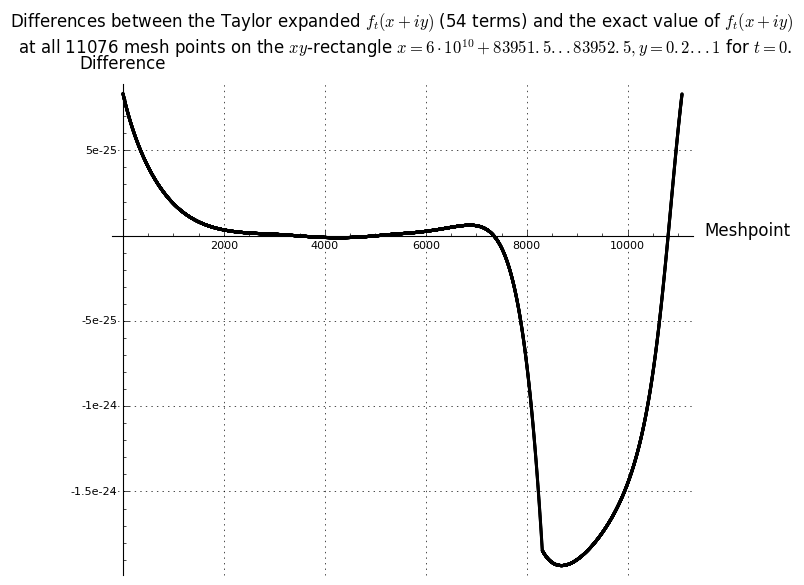
\includegraphics[width=0.7\linewidth]{BarrieraccuracyTaylor}
  \caption{Achieved error term in the Taylor expansion at $t=0$. Target was set at $20$ decimal places accuracy.}\label{fig1}
\end{figure}

The derivative bounds determine the number of mesh points required on each $xy$-rectangle and in the $t$-direction. Figure \ref{fig2} ilustrates that these bounds have been chosen quite conservatively:

\begin{figure}[h!]
  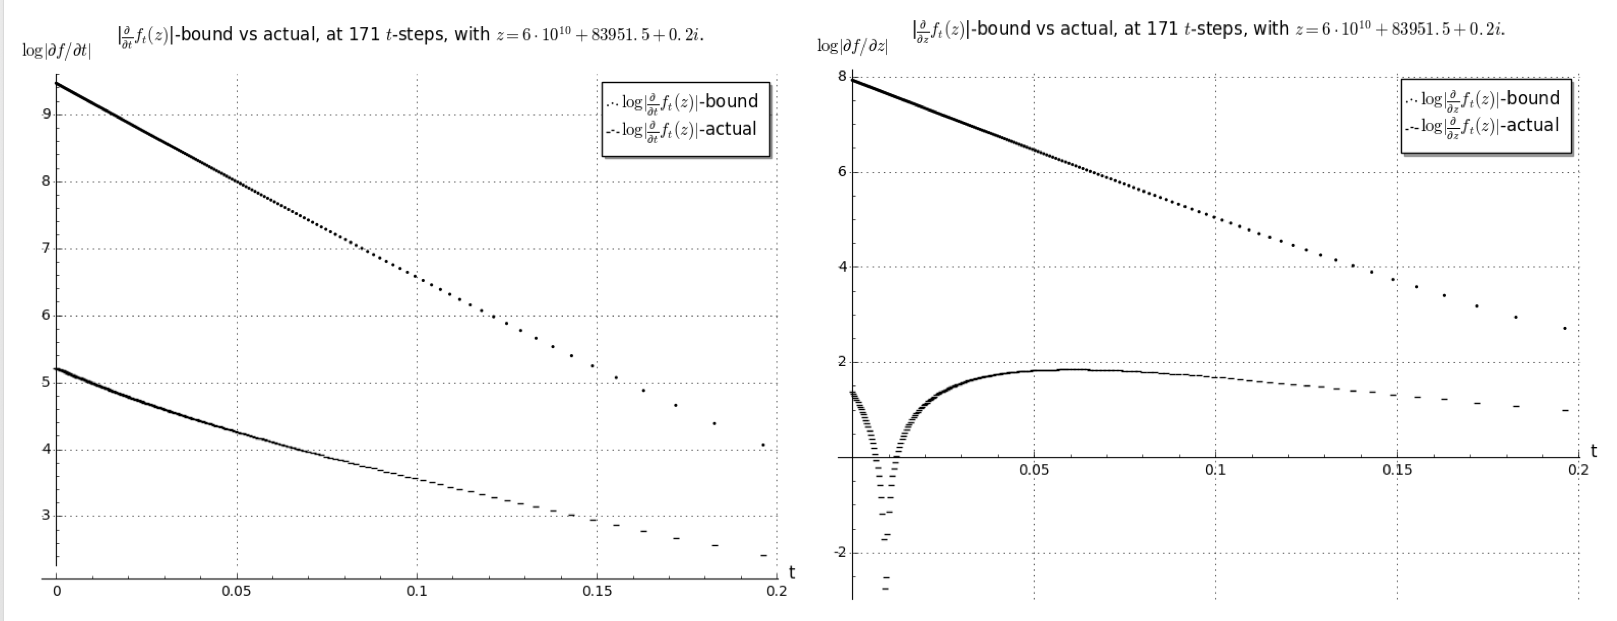
\includegraphics[width=1.0\linewidth]{Derivativebounds}
  \caption{Derivative bounds versus their actual values at all required steps of $t$.}\label{fig2}
\end{figure}

The number of rectangle mesh points varies with $t$ ranging from $11076$ at $t=0$ to $56$ at $t=0.195$; see Figure \ref{fig3}.

\begin{figure}[h!]
  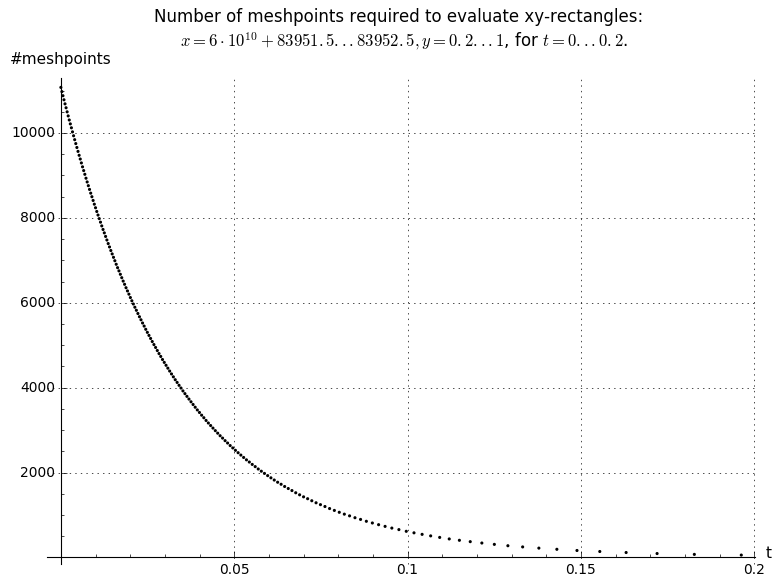
\includegraphics[width=0.7\linewidth]{Numberofmeshpoints}
  \caption{The number of mesh points required per rectangle for each step of $t$.}\label{fig3}
\end{figure}

The overall winding number for the barrier at this specific location came out at $0$. Figures \ref{fig4}, \ref{fig4a} show the winding process at $t=0, 0.2$ respectively. Due to the choice of the barrier location and the small barrier width compared to the wavelength in the $x$ variable, little oscillation is expected to occur in each rectangle.

\begin{figure}[h!]
  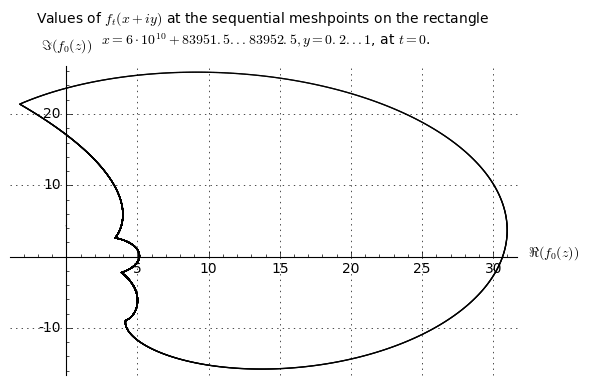
\includegraphics[width=0.7\linewidth]{Windingprocess}
  \caption{Winding the rectangle at $t=0$.}\label{fig4}
\end{figure}

\begin{figure}[ht!]
  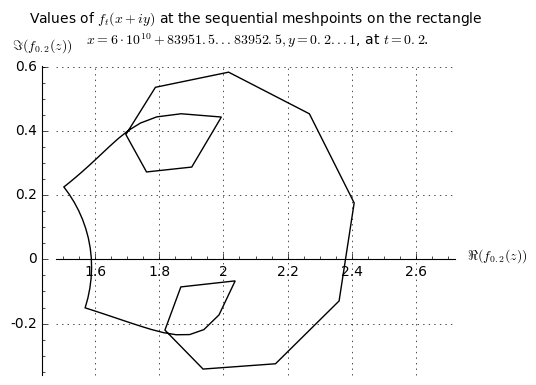
\includegraphics[width=0.7\linewidth]{Windingprocess_t02}
  \caption{Winding the rectangle at $t=0.2$.}\label{fig4a}
\end{figure}

The code for implementing these computations may be found in the directory

\centerline{\tt dbn\_upper\_bound/arb}

in the github repository \cite{github}.

\subsection{Proof of claim (b)}\label{b-bound}

Fix $t=0.2$, and let $R$ denote the rectangle
$$ R \coloneqq \{ x+iy: 0.2 \leq y \leq 1; x \geq X_0 - 0.5; N \leq N_1 \}.$$
We wish to show that the holomorphic function $H_t(x+iy)/B_t(x+iy)$ does not vanish in this rectangle.  We would like to establish this by the argument principle, however this turns out to be difficult to accomplish due to the oscillation in $H_t(x+iy)/B_t(x+iy) \approx f_t(x+iy)$ indicated by the heuristic \eqref{oscil}.  To damp out this oscillation, we introduce an\footnote{In the literature one also sees other choices of mollifier than this Euler product used, for instance to control the extreme values of Dirichlet polynomials; however our numerical experimentations with alternative mollifiers to $f_t(x+iy)$ turned out to give inferior results for our application.} ``Euler mollifier''
$$ E_{t,5}(x+iy) \coloneqq \prod_{p \leq 5} \left( 1 - \frac{b_p^t}{p^{s_*}}\right),$$
where $s_*$ is given by \eqref{sn-def} the choice to use the first three primes $2,3,5$ was obtained after significant trial and error as giving the best numerical results in this range of $t,x,y$.  We have the upper bound
$$
|E_{t,5}(x+iy)| \leq \prod_{p \leq 5} \left(1 + \frac{b_p^t}{p^{\mathrm{Re} s_*}} \right).
$$
When $N \geq N_0$, $0.2 \leq y \leq 1$ and $t = 0.2$, one easily verifies from \eqref{res-bound} that
$$ \mathrm{Re} s_* \geq 1.7143 $$
and hence
$$ |E_{t,5}(x+iy)| \leq 1.635 $$ % 1.705 at p=7
In particular, by Proposition \ref{sweep} we have
$$ E_{t,5}(x+iy) \frac{H_t(x+iy)}{B_t(x+iy)} = E_{t,5}(x+iy) f_t(x+iy) + O_{\leq}( 2.05 \times 10^{-3} ).$$  % 2.14 at p=7
The left-hand side remains holomorphic in $x+iy$ (even though $f_t(x+iy)$ has jump discontinuities).  Thus, by the argument principle, it will suffice to show that the left-hand side avoids the negative real axis $(-\infty,0]$ as $x+iy$ traverses the boundary $\partial R$ of the rectangle $R$.  In other words, it will suffice to show that
\begin{equation}\label{star}
 \mathrm{dist}( E_{t,5}(x+iy) f_t(x+iy), (-\infty,0]) > 2.05 \times 10^{-3}
\end{equation}
for $x+iy \in\partial R$.
For future reference we also observe that for any $x+iy \in R$,
the magnitude of $E_{t,5}(x+iy)$ can be bounded below by
\begin{equation}\label{et5-lower}
 |E_{t,5}(x+iy)| \geq \prod_{p \leq 5} \left(1 - \frac{b_p^t}{p^{\mathrm{Re} s_*}} \right) \geq 0.534 
\end{equation} %  0.512 when p=7
and the argument has magnitude at most
\begin{equation}\label{et5-phase}
|\mathrm{arg}(E_{t,5}(x+iy))| \leq \sum_{p \leq 5} \sin^{-1} \frac{b_p^t}{p^{\mathrm{Re} s_*}} \leq 0.553. 
\end{equation} % 0.595 when p=7

Of the four sides of the rectangle $\partial R$, the required estimate \eqref{star} will hold with significant room to spare, and we can proceed using rather crude estimates.  We first attend to the right edge of $\partial R$, in which $N = N_1$.  
From \eqref{ft0} we have
$$
f_t(x+iy) = 1 + O_{\leq}( 0.955 )$$
in this region.  In particular $f_t(x+iy)$ has argument of magnitude at most $\sin^{-1} 0.955 \leq 1.27$.  Combining this with \eqref{et5-lower}, \eqref{et5-phase}, we conclude that $E_{t,5}(x+iy) f_t(x+iy)$ has magnitude at least $0.024$ and argument at most $1.823$ in magnitude, giving the claim \eqref{star} on this side from elementary trigonometry.

Now we attend to the left edge of $\partial R$, in which $x = X_0 - 0.5$ and $0.2 \leq y \leq 1$.  From the calculations for part (a) (see in particular Figure \ref{fig4a}) one can verify that (for instance) $|f_t(x+iy)| \geq 1$ and $|\mathrm{arg} f_t(x+iy)| \leq \frac{\pi}{2}$ in this region.  Combining this with \eqref{et5-lower}, \eqref{et5-phase}, we conclude that $E_{t,5}(x+iy) f_t(x+iy)$ has magnitude at least $0.534$ and argument at most $2.13$ in magnitude, again giving the claim \eqref{star} on this side from elementary trigonometry.

Now we attend to the upper edge of $\partial R$, in which $N_0 \leq N \leq N_1$ and $y=1$.  From \eqref{res-bound} one now has
$$ \mathrm{Re} s_* \geq 2.1143.$$
In particular\footnote{The sum $\sum_{n=2}^{N_1} \frac{b_n^t}{n^{2.1143}}$ can be numerically computed directly, but one could also use Lemma \ref{largen} (using for instance $N_0 = 69098$) to obtain a usable upper bound as well.  Similarly for the other sums of this type that appear in this argument.}
$$ \sum_{n=1}^N \frac{b_n^t}{n^{s_*}} = 1 + O_{\leq}\left( \sum_{n=2}^{N_1} \frac{b_n^t}{n^{2.1143}} \right) = 1 + O_{\leq}( 0.7 ).$$
Meanwhile, from \eqref{gamma-bound} one has
$$ |\gamma| \leq e^{0.02} \left( \frac{x}{4\pi} \right)^{-1/2} \leq 1.03 N^{-1}$$
and from \eqref{kappa-bound} one has
$$ |\kappa| \leq \frac{ty}{2(x-6)} \leq 4 \times 10^{-13}$$
and hence
$$ |\gamma| \frac{n^y}{n^{s_* + \kappa}} = O_{\leq}( \frac{1.03}{N n^{1.1142}} )$$
and
$$   \gamma \sum_{n=1}^N n^y \frac{b_n^t}{n^{\overline{s_*} + \kappa}} = O_{\leq}\left( \sum_{n=2}^{N_0} \frac{1.03 b_n^t}{N_0 n^{1.1142}} + \sum_{n=N_0+1}^{N_1} \frac{1.03 b_n^t}{n^{2.1142}} \right) = O_{\leq}( 0.1 )$$
and hence
$$ f_t(x+iy) = 1 + O_{\leq}(0.8).$$
In particular $f_t(x+iy)$ has magnitude at least $0.2$ and argument at most $0.928$ in magnitude, hence $E_t(x+iy) f_t(x+iy)$ has magnitude at least $0.1068$ and argument at most $1.481$, at which point the claim follows from elementary trigonometry.

It remains to attend to the lower edge of $\partial R$, in which $N_0 \leq N \leq N_1$ and $y=0.2$.  This is by far the most delicate side of the rectangle for the purposes of verifying \eqref{star}.  We will split the range $[N_0,N_1]$ into a number of subintervals $[N_-,N_+]$ and obtain a uniform lower bound for $\mathrm{dist}( E_{t,5}(x+iy) f_t(x+iy), (-\infty,0])$ when $N$ is in one of these subintervals $[N_-,N_+]$.

Fix $[N_-,N_+] \subset [N_0,N_1]$, suppose that $N \in [N_-,N_+]$, and write $s_* = \sigma + iT$.  We first deal with the $\kappa$ term in the definition of $f_t(x+iy)$ by writing
$$ n^{-\kappa} = 1 + O_{\leq}( n^{|\kappa|}-1)$$
and hence
\begin{equation}\label{ftxy}
 f_t(x+iy) = \sum_{n=1}^N \frac{b_n^t}{n^{\sigma+iT}} + \gamma \sum_{n=1}^N n^y \frac{b_n^t}{n^{\sigma-iT}}
+ O_{\leq}\left( |\gamma| \sum_{n=1}^N n^y \frac{b_n^t}{n^\sigma} (n^{|\kappa|}-1) \right).
\end{equation}
In particular, using \eqref{gamma-bound} to bound
\begin{align*}
|\gamma| &\leq e^{0.02y} (x_N/4\pi)^{-y/2} \\
&\leq e^{0.004} \left(N^2 - \frac{1}{80}  \right)^{-0.1} \\
&\leq 1.005 N^{-0.2} \\
&\leq 1.005 N_-^{-0.2}.
\end{align*}
we have
$$ E_{t,5}(x+iy) f_t(x+iy) = E_{t,5}(x+iy) \sum_{n=1}^N \frac{b_n^t}{n^{\sigma+iT}} + O_{\leq}\left( 1.005 |E_{t,5}(x+iy)| 
\left|\sum_{n=1}^N (n/N_-)^{0.2} \frac{b_n^t}{n^{\sigma-iT}}\right| \right)
+ O_{\leq}( Z )$$
where
$$ Z \coloneqq 1.644 \sum_{n=1}^N (n/N)^{0.2} \frac{b_n^t}{n^\sigma} (n^{|\kappa|}-1).$$
We can write
$$ E_{t,5}(x+iy) = \sum_{d|D} \frac{\lambda_d}{d^{\sigma+iT}}$$
where $D \coloneqq 2 \times 3 \times 5$ and
$$ \lambda_d \coloneqq \prod_{p|d} (-b_p^t).$$
As a consequence, we have
$$ E_{t,5}(x+iy) \sum_{n=1}^N \frac{b_n^t}{n^{\sigma+iT}} = \sum_{n=1}^{DN} \frac{\beta_{n}}{n^{\sigma+iT}}$$
where
$$ \beta_{n} \coloneqq \sum_{d|n,D} \lambda_d b_{n/d}^t.$$
Thus for instance $\beta_1 = 1$ and $\beta_p = 0$ for $p=2,3,5$, so that the Dirichlet series $\sum_{n=1}^{DN} \frac{\beta_n}{n^{\sigma+iT}}$ is expected to experience less oscillation than the series $\sum_{n=1}^N \frac{b_n^t}{n^{\sigma+iT}}$.

The product of $E_{t,5}(x+iy)$ and $\sum_{n=1}^N (n/N_-)^{0.2} \frac{b_n^t}{n^{\sigma-iT}}$ is not favorable due to the negative sign in the $\sigma-iT$ exponent.  But since $|z| |w| = |z \overline{w}|$, we have
\begin{align*}
1.005 |E_{t,5}(x+iy)| \left|\sum_{n=1}^N (n/N_-)^{0.2} \frac{b_n^t}{n^{\sigma-iT}}\right|  &=
1.005 \left|E_{t,5}(x+iy) \sum_{n=1}^N (n/N_-)^{0.2} \frac{b_n^t}{n^{\sigma+iT}}\right|  \\
&= \left|\sum_{n=1}^{DN} \frac{N_-^{-0.2} \alpha_{n}}{n^{\sigma+iT}}\right|
\end{align*}
where
$$ \alpha_{n} \coloneqq 1.005 \sum_{d|n,D} \lambda_d (n/d)^{0.2} b_{n/d}^t.$$
Note that the coefficients $\alpha_{n}, \beta_n$ are both real.  We now have
\begin{equation}\label{ets}
 E_{t,5}(x+iy) f_t(x+iy) = \sum_{n=1}^{DN} \frac{\beta_n}{n^{\sigma+iT}} + O_{\leq}\left( \left|\sum_{n=1}^{DN} \frac{N_-^{-0.2} \alpha_{n}}{n^{\sigma+iT}}\right| \right) + O_{\leq}(Z).
\end{equation}
A naive application of the triangle inequality (using $\beta_1=1$) would give the lower bound
\begin{equation}\label{eft}
 \mathrm{dist}(E_{t,5}(x+iy) f_t(x+iy), (-\infty,0]) \geq 1 - N_-^{-0.2} \alpha_{1} - \sum_{n=2}^{DN} \frac{|\beta_n| + |N_-^{-0.2} \alpha_{n}|}{n^{\sigma}} - Z.
\end{equation}
As it turns out, this bound is not quite strong enough to be satisfactory for the numerical ranges of parameters we need.  To do better we need to exploit the fact that when the sum $\sum_{n=1}^{DN} \frac{\beta_n}{n^{\sigma+iT}}$ exhibits significant cancellation, then the sum $\sum_{n=1}^{DN} \frac{N^{-0.2} \alpha_{n}}{n^{\sigma+iT}}$ will also. The key tool here is

\begin{lemma}[Improved triangle inequality]  We have
$$ \mathrm{dist}(E_{t,5}(x+iy) f_t(x+iy), (-\infty,0]) \geq 1 - N_-^{-0.2} \alpha_{1} - \sum_{n=2}^{DN} \frac{\max(|\beta_n-N_-^{-0.2} \alpha_{n}|, \frac{1-N_-^{-0.2} \alpha_{1}}{1+N_-^{-0.2} \alpha_{1}} |\beta_n+N_-^{-0.2} \alpha_{n}|)}{n^{\sigma}} - Z.$$
\end{lemma}

\begin{proof}
Write 
$$ Y \coloneqq \sum_{n=2}^{DN} \frac{\max(|\beta_n-N_-^{-0.2} \alpha_n|, \frac{1-N_-^{-0.2} \alpha_1}{1+N_-^{-0.2} \alpha_1} |\beta_n+N_-^{-0.2} \alpha_n|)}{n^{\sigma}}.$$
We may assume that $N_-^{-0.2} \alpha_1+Y < 1$, otherwise the claim is trivial.  By \eqref{ets} and convexity, it suffices to show that
$$
\mathrm{dist}( \sum_{n=1}^{DN} \frac{\beta_n + e^{i\theta} N_-^{-0.2} \alpha_n}{n^{\sigma+iT}}, (-\infty,0]) \geq 1 - N_-^{-0.2} \alpha_1 - Y$$
for all phases $\theta \in \R$.  We may write
\begin{align*}
\sum_{n=1}^{DN} \frac{\beta_n + e^{i\theta} N_-^{-0.2} \alpha_n}{n^{\sigma+iT}} &= 1 + e^{i\theta} N_-^{-0.2} \alpha_1 + O_{\leq}\left( \sum_{n=2}^{DN}
\frac{|\beta_n + e^{i\theta} N_-^{-0.2} \alpha_n|}{n^{\sigma}} \right) \\
&=
(1 + e^{i\theta} N_-^{-0.2} \alpha_1) \left(1 + O_{\leq}\left( \sum_{n=2}^{DN}
\frac{|\beta_n + e^{i\theta} N_-^{-0.2} \alpha_n|/|1+e^{i\theta} N_-^{-0.2} \alpha_1|}{n^{\sigma}} \right) \right).
\end{align*}
By the cosine rule, we have
$$ \left(|\beta_n + e^{i\theta} N_-^{-0.2} \alpha_n| / |1 + e^{i\theta} N_-^{-0.2} \alpha_1|\right)^2 = \frac{\beta_n^2 + N_-^{-0.2} \alpha_n^2 + 2 N_-^{-0.2} \alpha_n \beta_n \cos \theta}{1 + N_-^{-0.2} \alpha_1^2 + 2 N_-^{-0.2} \alpha_1 \cos \theta}.$$
This is a fractional linear function of $\cos \theta$ with no poles in the range $[-1,1]$ of $\cos \theta$.  Thus this function is monotone on this range and attains its maximum at either $\cos \theta=+1$ or $\cos \theta = -1$.  We conclude that
$$ \frac{|\beta_n + e^{i\theta} N_-^{-0.2} \alpha_n|}{|1 + e^{i\theta} N_-^{-0.2} \alpha_1|} \leq \max\left( \frac{|\beta_n-N_-^{-0.2} \alpha_n|}{1-N_-^{-0.2} \alpha_1}, \frac{|\beta_n+N_-^{-0.2} \alpha_n|}{1+N_-^{-0.2} \alpha_1} \right)$$
and thus
$$ \sum_{n=2}^{DN} \frac{|\beta_n + e^{i\theta} N_-^{-0.2} \alpha_n|/|1+e^{i\theta} N_-^{-0.2} \alpha_1|}{n^{\sigma}} \leq \frac{1}{1-N_-^{-0.2} \alpha_1} Y.$$
We conclude from the triangle inequality that
$$ \sum_{n=1}^{DN} \frac{\beta_n + e^{i\theta} N_-^{-0.2} \alpha_n}{n^{\sigma+iT}} = 1 + e^{i\theta} N_-^{-0.2} \alpha_1 + O_{\leq}\left( \frac{|1+e^{i\theta} N_-^{-0.2} \alpha_1|}{1-N_-^{-0.2} \alpha_1} Y \right).$$
By further application of the triangle inequality
\begin{align*}
\mathrm{dist}( \sum_{n=1}^{DN} \frac{\beta_n + e^{i\theta} N_-^{-0.2} \alpha_n}{n^{\sigma+iT}}, (-\infty,0]) &\geq \mathrm{dist}( 1 + e^{i\theta} N_-^{-0.2} \alpha_1, (-\infty,0]) - \frac{|1+e^{i\theta} N_-^{-0.2} \alpha_1|}{1-N_-^{-0.2} \alpha_1} Y \\
&= |1 + e^{i\theta} N_-^{-0.2} \alpha_1| - \frac{|1+e^{i\theta} N_-^{-0.2} \alpha_1|}{1-N_-^{-0.2} \alpha_1} Y  \\
&= |1 + e^{i\theta} N_-^{-0.2} \alpha_1| \left(1 - \frac{Y}{1-N_-^{-0.2} \alpha_1} \right) \\
&\geq (1-N_-^{-0.2} \alpha_1) \left(1 - \frac{Y}{1-N_-^{-0.2} \alpha_1} \right) \\
&= 1 - N_-^{-0.2} \alpha_1 - Y
\end{align*}
as desired, where we have used the fact that $1+e^{i\theta} N_-^{-0.2} \alpha_1$ lies to the right of the imaginary axis (so that the closest element of $(-\infty,0]$ is the origin).
\end{proof}

Bounding $DN \leq DN_+$, we see that in order to establish \eqref{star} in the range $N \in [N_-, N_+]$, it suffices to verify the inequality
$$ 1 - N_-^{-0.2} \alpha_1 - \sum_{n=2}^{DN_+} \frac{\max(|\beta_n-N_-^{-0.2} \alpha_n|, \frac{1-N_-^{-0.2} \alpha_1}{1+N_-^{-0.2} \alpha_1} |\beta_n+N^{-0.2} \alpha_n|)}{n^{\sigma}} - Z
\geq 2.14 \times 10^{-3}.$$
From \eqref{res-bound}, \eqref{xnn} one has 
\begin{align*}
 \sigma &\geq \frac{1+y}{2} +\frac{t}{4} \log \frac{x_N}{4\pi} - \frac{t}{2x_N^2} \left(1-3y+\frac{4y(1+y)}{x_N^2}\right)_+ \\
&= 0.6 + \frac{1}{20} \log \frac{x_N}{4\pi} - \frac{1}{10 x_N^2} \left( 0.4 + \frac{0.96}{x_N^2} \right) \\
&= 0.6 + \frac{1}{20} \log (N^2 - \frac{1}{80}) - \frac{1}{10 x_{N_0}^2} \left( 0.4 + \frac{0.96}{x_{N_0}^2} \right) \\
&\geq \sigma_{N_-}
\end{align*}
where
$$ \sigma_{N_-} \coloneqq 0.599 + \frac{1}{10} \log N_- $$
while from \eqref{kappa-bound}, \eqref{xnn} one has
$$ |\kappa| \leq \frac{ty}{2(x_N-6)} \leq \frac{0.02}{x_{N_0}-6} \leq 4 \times 10^{-13}$$
and hence it suffices to show that
$$ F_{N_-,N_+} - Z_{N_-,N} \geq 2.14 \times 10^{-3}$$
where
$$ F_{N_-,N_+} \coloneqq 1 - N_-^{-0.2} \alpha_1 - \sum_{n=2}^{DN_+} \frac{\max(|\beta_n-N_-^{-0.2} \alpha_n|, \frac{1-N_-^{-0.2} \alpha_1}{1+N_-^{-0.2} \alpha_1} |\beta_n+N_-^{-0.2} \alpha_n|)}{n^{\sigma_{N_-}}}$$
and
$$ Z_{N_-,N} \coloneqq 1.644 \sum_{n=1}^N (n/N)^{0.2} \frac{b_n^t}{n^{\sigma_{N_-}}} (n^{4 \times 10^{-13}}-1).$$
Since $\sigma_{N_-} \geq 1.714$, we may crudely bound
$$ Z_{N_-,N} \leq 1.644 \sum_{n=1}^{N_1} \frac{b_n^t}{n^{1.714}} (n^{4 \times 10^{-13}}-1) \leq 10^{-10}$$
so it will suffice to show that
$$ F_{N_-,N_+} \geq 2.15 \times 10^{-3}$$
for a collection of intervals $[N_-,N_+]$ covering $[N_0, N_1]$.  This can be done by \emph{ad hoc} numerical experimentation; for instance, one can calculate that
\begin{align*}
F_{69098, 8 \times 10^4} &= 0.0263\dots \\
F_{8 \times 10^4, 1.1 \times 10^5} &= .0470\dots \\
F_{1.1 \times 10^5, 2.2 \times 10^5} &= 0.093\dots \\
F_{2.2 \times 10^5, 1.5 \times 10^6} &= 0.060\dots .
\end{align*}
